\documentclass{article}

\usepackage{project_440_550}
% Please submit it as is here, with line numbers.
% If you'd like a "less draft"-looking version for your website or something after:
%     \usepackage[final]{project_440_550}   % keeps the footer but kills line numbers,
%     \usepackage[preprint]{project_440_550}   % removes both


\usepackage[utf8]{inputenc} % allow utf-8 input
\usepackage[T1]{fontenc}    % use 8-bit T1 fonts

\usepackage[USenglish]{babel}  % there's a "canadian" option, but it's an alias for USenglish,
                               % and for some reason it makes csqoutes behave differently...
\usepackage{csquotes}       % smarter handling of quotes (used by biblatex)
\usepackage{graphicx}
\usepackage{booktabs}       % professional-quality tables
\usepackage{amsfonts}       % blackboard math symbols
\usepackage{nicefrac}       % compact symbols for 1/2, etc.
\usepackage{microtype}      % microtypography
\usepackage{xcolor}         % colors
\usepackage{hyperref}       % hyperlinks
\usepackage{url}            % simple URL typesetting
\usepackage{amsmath}
\usepackage{float}

% I recommend the biblatex package.
% If you hate it for some reason, though, you can use natbib instead:
% comment out this block and uncomment the next one.
\usepackage[capitalize,noabbrev]{cleveref}
\usepackage[style=authoryear,maxbibnames=30,natbib]{biblatex}
\addbibresource{refs.bib}
\renewbibmacro{in:}{}  % drops a silly "In:" from biblatex format
\DeclareDelimFormat{nameyeardelim}{\addspace} % remove a comma i dislike, doesn't matter
\DeclareNameAlias{sortname}{given-family}  % avoid kinda-weird bib printing order

%\usepackage[round]{natbib}
%\newcommand{\printbibliography}{\bibliographystyle{plainnat}\bibliography{refs}}


\usepackage[capitalize,noabbrev]{cleveref}


\title{When Do Diffusion Transformers Outperform U-Nets?}


% The \author macro works with any number of authors. There are two commands
% used to separate the names and addresses of multiple authors: \And and \AND.
%
% Using \And between authors leaves it to LaTeX to determine where to break the
% lines. Using \AND forces a line break at that point. So, if LaTeX puts 3 of 4
% authors names on the first line, and the last on the second line, try using
% \AND instead of \And before the third author name.

\author{%
Arshvir Sandhu\\
  \texttt{arshvirs@student.ubc.ca}
  \And
  Gunbir Baveja\\
  \texttt{gbaveja@student.ubc.ca}
  \And
  Parvin Aliyeva\\
  \texttt{paliyeva@cs.ubc.ca}
}

\begin{document}
\maketitle


\begin{abstract}
    
    % here goes a potential abstract
    Diffusion transformers (DiT) have recently emerged as an alternative to U-Nets for denoising in diffusion models, but their reported improvements are typically demonstrated at large scale, making it unclear whether the gains stem from the architecture itself or from scale.
    We present a controlled comparison between a convolutional U-Net and a patch-based diffusion transformer, trained with matched parameter budgets on CIFAR-10.
    Beyond standard generation quality, we evaluate both architectures under structured corruptions: patch masking, block occlusion, and stripe removal. 
    These corruptions degrade local cues and demand long-range spatial reasoning from the denoiser.
    We additionally perform ablation studies over transformer patch size and model depth.
    Our results offer insight into the conditions under which global self-attention provides a genuine advantage over convolutional locality for the denoising task.
    
\end{abstract}


\section{Introduction}

Diffusion models learn to generate data by reversing a gradual corruption process: given a clean sample, Gaussian noise is incrementally added until the original signal is destroyed, and a neural network is trained to undo each step of this corruption \citep{ho2020ddpm}. 
Since their introduction, diffusion models have become a dominant paradigm in image generation, producing samples that rival or surpass those of generative adversarial networks while offering more stable training dynamics \citep{dhariwal2021diffusionbeat}.

The architectural backbone of many early diffusion models is the U-Net \citep{ronneberger2015unet}, a convolutional encoder-decoder with skip connections originally developed for biomedical image segmentation.
In diffusion models, its convolutional structure gives a natural bias toward local spatial patterns, since each layer operates over a limited receptive field and broader context is built up gradually through downsampling.
This seems well-suited for denoising, where much of the important structure is local, and U-Net-based diffusion models have achieved strong results across many benchmarks \citep{ho2020ddpm, rombach2022ldm}.

% transformers now
% question if they're actually better, or is it all just scaling
% small, controlled setting. justify experimental setup
% aim and hypothesis 
% outline the experiments 
% ight bet
More recently, several works have explored transformer-based alternatives. 
Diffusion Transformer (DiT) \citep{peebles2023dit} replaces the U-Net with a patch-based transformer using self-attention and reports very strong results at scale. 
U-ViT \citep{bao2023uvit} also showed compettive performance using a transformer backbone with skip connections. 
More recent systems such as Stable Diffusion 3 \citep{esser2024sd3} have also moved in this direction. 


This raises a natural question: are transformers structurally better denoisers, or do they mainly benefit from scaling well?
Much of the evidence so far comes from huge models trained on massive datasets, making it difficult to separate architectural effects from scaling effects. In this project, we study this question in a small and controlled setting, keeping the diffusion setup, optimizer, training objective, and parameter count fixed while varying only the denoiser architecture. Specifically, we compare a standard U-Net against a patch-based diffusion transformer trained on CIFAR-10 \citep{krizhevsky2009cifar}, with the goal of isolating whether architectural inductive biases drive the performance differences reported in the literature rather than scale.


Beyond measuring FID, we also probe whether transformers naturally benefit from self-attention that models long-range dependencies directly as opposed to U-Nets that use downsampling. This factor may be especially relevant when local information is absent or ambiguous.  


% We also want to look beyond standard sample quality. 
% One possible advantage of transformers is that self-attention can model long-range dependencies directly, while U-Nets build this up more indirectly through downsampling.
% We hypothesize this might matter especially when local information is missing.

To test this, we evaluate both models under structured corruptions before adding diffusion noise. 
More specifically, we mask contiguous patches, remove large blocks, or erase alternating stripes, and then test how well the models reconstruct the original image.
The goal is to create settings where recovering the image may require more global reasoning. If transformers benefit significantly from global receptive fields, the effect should be more pronounced under these corruptions.

The paper focuses on three key contributions:
\begin{enumerate}
    \item A controlled comparison of U-Net and DiT denoisers on CIFAR-10 under roughly matched parameter budgets.
    \item A structured-corruption evaluation setup for testing robustness under long-range reconstruction challenges.
    \item Ablations varying transformer patch size and depth to study what aspects of the architecture matter most.
\end{enumerate}

Together, these experiments are designed to disentangle the role of architectural inductive biases from the effects of scale that dominate the existing literature. If DiT outperforms under these structured corruptions, that would support the idea that attention provides an architectural advantage beyond scaling. Otherwise, the results may suggest the advantage seen in prior work comes mainly from large-scale training.

\section{Related Work}
\label{sec:related}

\paragraph{Diffusion models.}
Denoising diffusion probabilistic models were introduced by \citet{ho2020ddpm} who showed that a U-Net trained to reverse a Gaussian noising process could generate high-quality images.
Subsequent work improved sample quality through better noise schedules and architectural refinements \citep{nichol2021improved}, and \citet{dhariwal2021diffusionbeat} demonstrated that diffusion models could surpass GANs on class-conditional ImageNet generation by using larger U-nets with additional attention layers.
Latent diffusion models \citep{rombach2022ldm} reduced the computational cost by applying the diffusion process in a compressed latent space, enabling high-resolution generation with moderate compute.
Throughout this line of work, the convolutional U-Net remained the default denoiser architecture.
Our project uses the same discrete-time DDPM framework and training objective, but focuses on comparing the denoiser backbone rather than improving the surrounding pipeline.

\paragraph{Transformer-based denoisers.}
% DiT stuff, key finding
% U-ViT stuff, key improvement
% DiffiT stuff, further improvement
% distinction from these methods
\citet{peebles2023dit} proposed the Diffusion Transformer (DiT), which replaces the U-Net with a vision transformer operating on \emph{patchified} latent representations. 
They showed that increasing transformer compute, through depth, width, or token count, consistently improved FID, with larger DiT models achieving state-of-the-art results on ImageNet.
Concurrently, \citep{bao2023uvit} introduced U-ViT, a transformer backbone with U-Net-style skip connections, and showed competitive or improved performance over convolutional U-Nets on benchmarks including unconditional CIFAR-10 generation.
DiffiT \citep{hatamizadeh2024diffit} further explored transformer-based diffusion using time-dependent self-attention, also reporting strong CIFAR-10 results in pixel space.
More recent models such as PixArt-$\alpha$ \citep{chen2024pixart} and Stable Diffusion 3 \citep{esser2024sd3} also use transformer backbones in large-scale text-to-image generation.

Our project differs from this line of work in two ways. First, rather than studying scaling benefits, we focus on whether transformers retain an advantage at small scale under roughly matched parameter budgets.
Second, prior work has not, to our knowledge, examined robustness under structured corruptions intended to probe long-range dependencies, which is one focus of our experiments.

\paragraph{Scaling studies.}
\citet{li2024scalability} conducted a controlled comparison of U-Net and transformer backbones for text-to-image diffusion under matched training conditions. 
They found transformer depth to be a parameter-efficient scaling direction, while also identifying efficient U-Net variants that remained competitive.
However, their experiments operate at much larger scales than we consider.
\citet{tian2024udit} proposed U-DiTs, which combine token downsampling with transformer blocks, and showed strong quality-efficieny tradeoffs.

These works are related to ours, but ask a somewhat different question: how to scale transformer diffusion models effectively, whereas we ask whether transformers help at all in a low-budget regime.

\paragraph{Inductive biases of CNNs and transformers.}
% dosovitsky study
% transformers bad cause large-scale pre-training required to match cnn performance
% vits and cnns [raghu] develop different representatinos
% transformers tend to capture global structure earlir
% transformers are more robust to corruptions, likely cause they model long-range dependencies
% what about generative settings though? 
The question of when transformers outperform convolutions has also been studied in discriminative settings.
\citet{dosovitskiy2021vit} showed that Vision Transformers often reque large-scale pre-training to match CNN performance, suggesting weaker inductive bias can be a disadvantage in low-data settings.
\citet{raghu2021vision} found that ViTs and CNNs develop different representations, with transformers tending to capture global structure earlier.
\citet{naseer2021intriguing} showed transformers can be more robust to some image corruptions, possibly due to their ability to model long-range dependencies. 

In generative settings, this question is less settled. \citet{park2022visiontransformer} studied interactions between attention and convolution and found self-attention may improve optimization in some settings.
% us now
Partly motivated by this line of work, our structured corruption experiments ask: if transformers do help with long-range dependencies, does it become more visible when local structure is disrupted?
% might need to fix this line above as it likely deviates from mark's comments on writing

\section{Method}
\label{sec:method}

\subsection{Diffusion Framework}

Both models are trained within a standard discrete-time DDPM framework \citep{ho2020ddpm}. 
Given a clean image $x_0$, the forward process produces a noisy image $x_t$ at timestep $t\in\{1,\ldots,T\}$ according to 
\begin{equation}
    x_t=\sqrt{\bar\alpha_t}x_0+\sqrt{1-\bar\alpha_t},\varepsilon,\quad\varepsilon\sim\mathcal N(0,I),
    \label{eq:forward}
\end{equation}
where $\bar\alpha_t = \prod_{s=1}^{t}(1-\beta_s)$ and $\{\beta_t\}_{t=1}^T$ is a linear noise schedule with $\beta_1=10^{-4}$ and $\beta_T=0.02$.
We use $T=500$ timesteps.
A denoising model $f_\theta(x_t,t)$ is trained to predict the added noise $\varepsilon$ by minimizing the objective
\begin{equation}
    \mathcal{L}(\theta)=\mathbb E_{x_0, \varepsilon, t}\bigl[\lVert\varepsilon-f_\theta(x_t,t)\rVert_2^2\bigr].
    \label{eq:loss}
\end{equation}
This objective is shared by both architectures; the only difference between the two experiments is the denoiser $f_\theta$ itself.

\subsection{U-Net Baseline}
Our U-Net follows the standard DDPM design. 
The encoder consists of residual blocks with group normalization and SiLU activations, organized across multiple resolution levels with channel widths determined by a base channel count and a set of multipliers.
Timestep information is injected by projecting a sinusoidal positional embedding through an MLP and adding it to the intermediate activations within each residual block.
A multi-head self-attention block is applied at the bottleneck resolution.
The decoder mirrors the encoder, with skip connections that concatenate encoder features at each resolution level.

We use a base channel width of $32$ with multipliers $(1,2,2)$, yielding channel widths of $32$, $64$, and $64$ at successively lower resolutions. 
The model operates at CIFAR-10's native $32 \times 32$ resolution.

\subsection{Diffusion Transformer}

Our DiT follows the design of \citep{peebles2023dit}.
The input image is split into non-overlapping $p\times p$ patches, each of which is linearly projected to produce a token embedding.
Learnable position embeddings are added, and the resulting sequence is processed by a stack of transformer blocks.
Each block consists of multi-head self-attention and an MLP with GeLU activation.
Timestep conditioning is injected via adaptive layer normalization with zero initialization (adaLN-Zero): the timestep embedding modulates the scale, shift, and gating parameters of each sub-layer, with all modulation parameters initialized to zero so that each block begins as the identity function.
The output tokens are linearly projected back to pixel space and rearranged into the original image layout.

We use a patch size of $4$ (yielding $8\times 8=64$ tokens for a $32\times 32$ image), a hidden dimension of $128$, $4$ transformer blocks, and $4$ attention heads.

\subsection{Training Protocol}

Both models are trained on the CIFAR-10 training set (50,000 images) with identical hyperparameters: AdamW optimizer with learning rate $2\times 10^{-4}$, batch size $128$, gradient clipping at norm $1.0$, and an exponential moving average (EMA) of model weights with decay $0.9999$.
% maybe too concise?
Training runs for $40$ epochs.
All reported results use the EMA model.
The only data augmentation is random horizontal flipping.
The U-Net has 1.30M trainable parameters and the DiT has 1.34M, ensuring a fair comparison at matched capacity.

\subsection{Structured Corruption Evaluation}

To test whether the transformer benefits more from global context, we evaluate both trained denoisers under a structured-corruption protocol.
Given a clean test image $x_0$, we: 
\begin{enumerate}
% divide image into patches, randomly turning them off
% add diffusion onise 
% apply denoiser to predict noise
% reconstruct the estimate of a clean image
% measure MSE? perhaps no need for this?
    \item Divide the image into a grid of $p_m\times p_m$ non-overlapping patches and randomly mask a fraction $r$ of them by setting their pixel values to zero, producing a corrupted image $\tilde x_0$.
    \item Add diffusion noise at a fixed evaluation timestep $t_{\text{eval}}=T/2$ to obtain $x_t=\sqrt{\bar\alpha_{t_\text{eval}}}\tilde x_0+\sqrt{1-\bar\alpha_{t_\text{eval}}}\varepsilon$.
    \item Apply the trained denoiser to predict the noise: $\hat\varepsilon=f_\theta(x_t,t_\text{eval})$.
    \item Reconstruct an estimate of the clean image: $\hat x_0=(x_t-\sqrt{1-\bar\alpha_{t_\text{eval}}}$.
    \item Measure reconstruction MSE separately in the \emph{masked} and \emph{unmasked} regions relative to the original clean image $x_0$.
\end{enumerate}
In our primary experiments, we use $p_m=8$ patches and $r=0.5$ (i.e., half of the $8\times 8$ patches are masked), and average results over multiple test batches.
The key quantity of interest is the MSE in the masked region: this measures how well the denoiser recovers content that was absent from the corrupted input. This requires integrating information from distant visible regions.

\subsection{Ablation Studies}

To understand which aspects of the transformer architecture matter most, we perform ablations on two quantities: (i)~ Patch size (2, 4, 8): controls the number of tokens and, consequently, the granularity of global attention. Smaller patches yield more tokens and finer spatial resolution but higher computational cost. (ii)~ Model depth (4, 6, 8 transformer blocks): controls the network's capacity for composing local and global features across layers.

For each ablation, we retrain the DiT variant under identical conditions and evaluate on both the standard denoising objective and the structured-corruption protocol.

\section{Experiments and Results}
\label{sec:experiments}

\subsection{Standard Denoising Comparison}

\Cref{fig:loss} shows the training loss curves over 40 epochs.
The U-Net converges faster and reaches a substantially lower final loss ($\approx 0.047$) than the DiT ($\approx 0.078$)
% not sure if we need to add this
, a relative gap of roughly 40\%.
The DiT begins at a much higher loss, likely due to the adaLN-Zero initialization, which causes each block to start as the identity, but drops rapidly within the first few epochs before plateauing.
Despite this, the gap persists throughout training, suggesting that at this scale the convolutional inductive biases (locality, translation equivariance, multi-resolution processing) provide a genuine advantage that the transformer cannot overcome through training alone.

This difference is also reflected in sample quality. Using $2048$ generated samples for evaluation, the U-Net obtains an FID of $247.45$, while the DiT obtains an FID of $340.18$.
Although both FID scores are high compared to fully trained diffusion models, which is expected given our small models and limited training budget, this comparison is still informative: under matched conditions, the U-Net produces substantially better samples than the DiT.
The U-Net's generated samples (see \Cref{app:samples}) show recognizable object structure, while the DiT samples are visibly noisier, consistent with the higher training loss.

\begin{figure}[t]
    \centering
    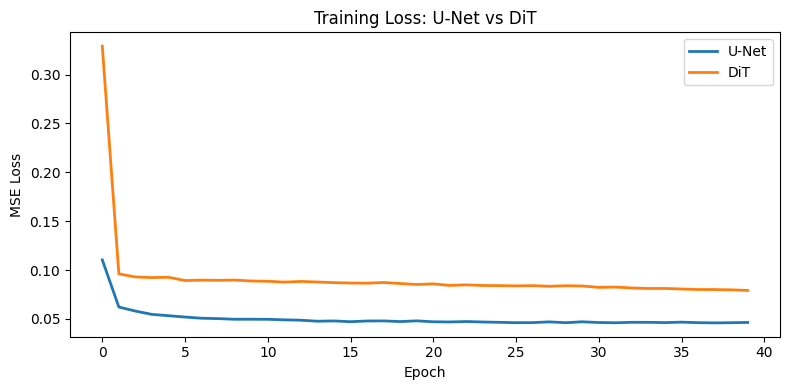
\includegraphics[width=0.55\linewidth]{figs/loss_curves.png}
    \caption{Training MSE loss over $40$ epochs on CIFAR-10. The U-Net converges faster and to a lower final loss than the DiT under matched training conditions (1.30M vs.\ 1.34M parameters).}
    \label{fig:loss}
\end{figure}

\begin{table}[t]
  \caption{Standard sample quality comparison using FID computed from 2048 generated samples. Lower is better.}
  \label{tab:fid}
  \centering
  \begin{tabular}{lc}
    \toprule
    Model & FID $\downarrow$ \\
    \midrule
    U-Net & \textbf{247.45} \\
    DiT   & 340.18 \\
    \bottomrule
  \end{tabular}
\end{table}

\subsection{Structured Corruption Results}

\Cref{tab:corruption} presents the main structured-corruption results.
Contrary to our hypothesis, the U-Net outperforms the DiT in \emph{both} the masked and unmasked regions, and by a substantial margin.
The U-Net achieves a masked-region MSE of $0.754$ compared to the DiT's $1.462$ (nearly twice as large) and the gap persists in the unmasked region ($0.260$ vs.\ $0.818$).

\begin{table}[t]
  \caption{Reconstruction MSE under structured patch corruption ($8\times8$ patches, 50\% mask ratio, noise at $t = T/2$). Lower is better. The U-Net outperforms the DiT in both masked and unmasked regions.}
  \label{tab:corruption}
  \centering
  \begin{tabular}{lcc}
    \toprule
    Model & Masked Region MSE & Unmasked Region MSE \\
    \midrule
    U-Net & \textbf{0.754} & \textbf{0.260} \\
    DiT   & 1.462 & 0.818 \\
    \bottomrule
  \end{tabular}
\end{table}

This result suggests that, at small scale, the U-Net's advantage is standard denoising transfers directly to the corruption settings: a model that is simply a better denoiser overall will also be better at recovering masked content, regardless of whether that recovery requires local or global reasoning.
\Cref{fig:recon} makes the contrast apparent: the U-Net's reconstructions, while noisy, preserve recognizable spatial structure and approximate color in the masked regions, whereas the DiT produces nearly incoherent outputs dominated by patch-level block artifacts, reflecting the same $4\times 4$ patch grid visible in its generated samples (see \Cref{fig:samples}).
An important caveat is that single-step denoising at a fixed noise level makes it difficult to disentangle whether the DiT's poor corruption reflects a fundamental inability to integrate global context or simply its weaker overall denoising capacity at this scale.

\begin{figure}[t]
    \centering
    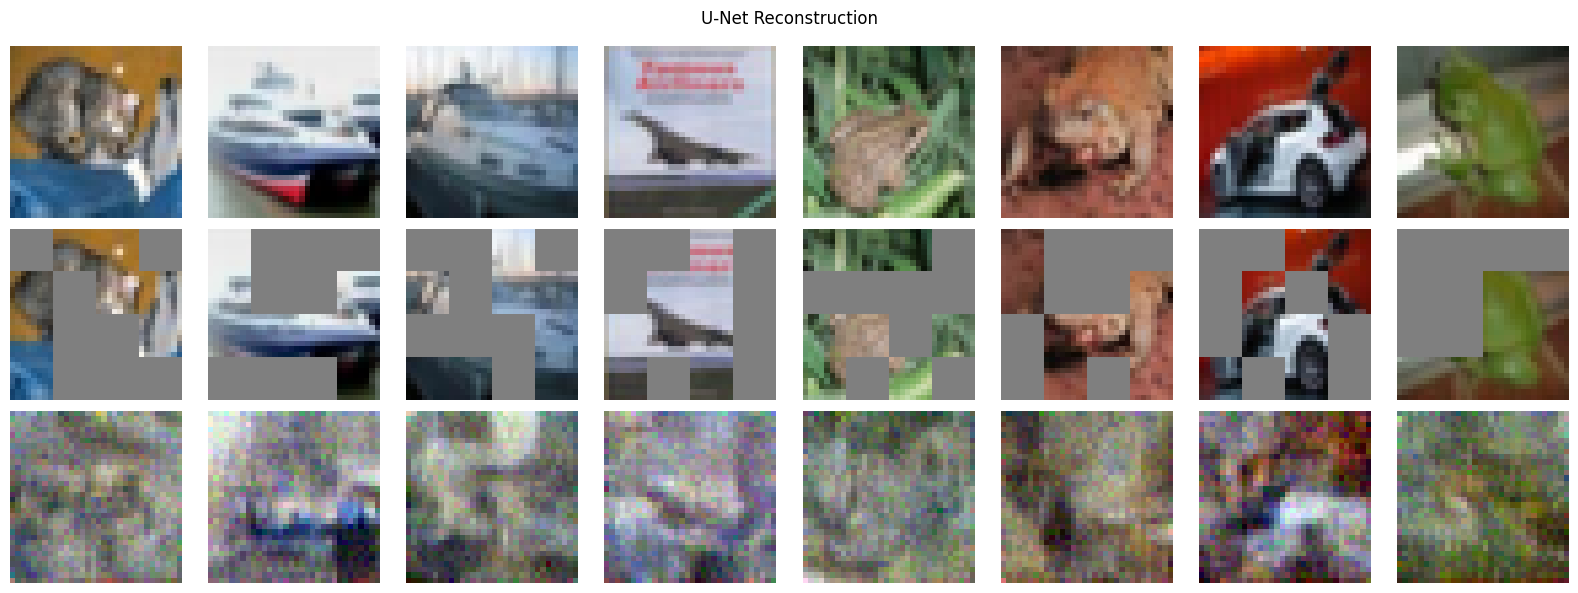
\includegraphics[width=0.8\linewidth]{figs/unet_recon.png}
    \vspace{0.3cm}
    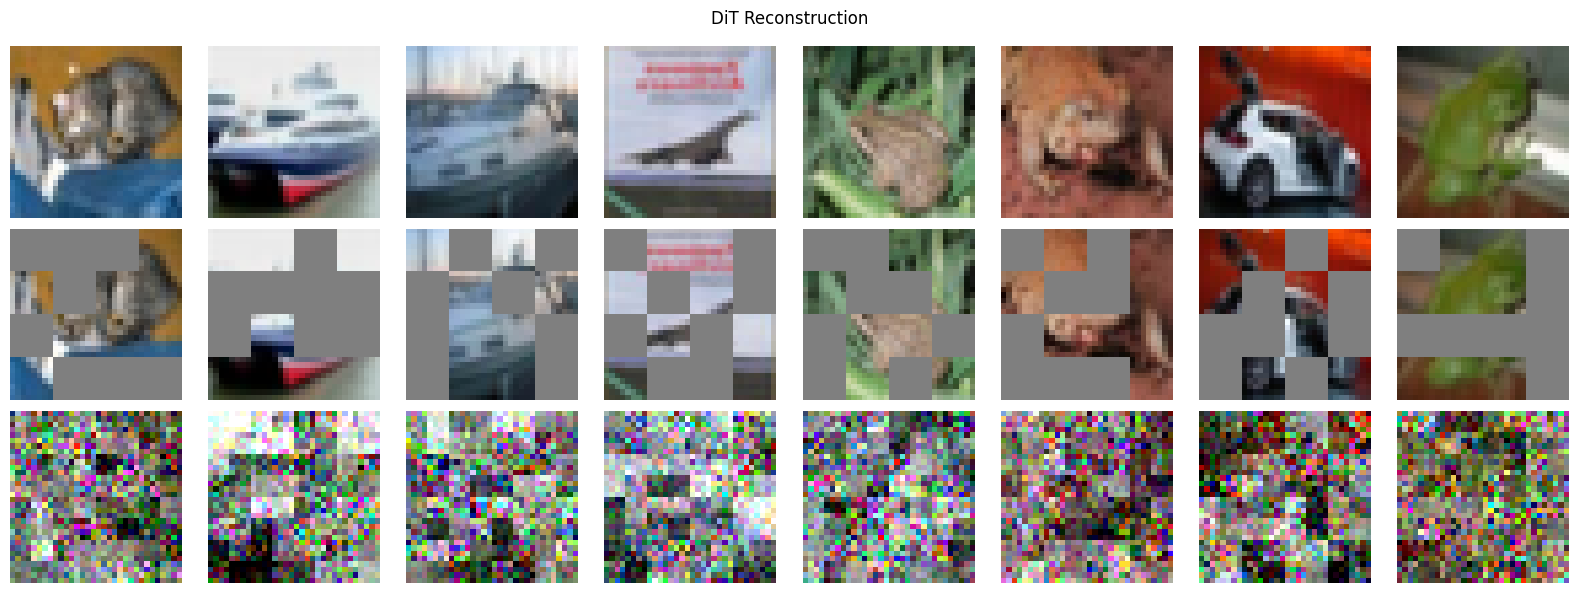
\includegraphics[width=0.8\linewidth]{figs/dit_recon.png}
    \caption{Reconstruction under structured corruption (50\% of $8\times 8$ patches masked, noise at $t=T/2$). Top panel: U-Net reconstructions preserve recognizable structure despite noise. Bottom panel: DiT outputs are nearly incoherent, with visible $4\times 4$ patch-grid artifacts reflecting the model's failure to learn meaningful spatial structure at this scale.}
    \label{fig:recon}
\end{figure}


\section{Discussion}
\label{sec:discussion}

Our main finding is that, at small scale, the convolutional U-Net provides a clear advantage over the diffusion transformer for both standard denoising and reconstruction under structured corruption.
The U-Net achieves a lower training loss, better FID, and substantially lower reconstruction error in both masked and unmasked regions.
This is a negative result with respect to our initial hypothesis as we expected the DiT's global self-attention to provide a measurable advantage when the denoising problem requires long-range context integration, but it is a meaningful one.

\paragraph{Why the U-Net wins at small scale.}
The convolutional architecture encodes strong inductive biases such as locality, translation equivariance, and multi-resolution feature extraction, that are well-matched to natural image structure.
At small model sizes and limited training, these biases effectively regularize the model, allowing it to learn useful features quickly.
The transformer, lacking these biases, must learn spatial structure entirely from data, which may require more capacity and training time than our regime provides.
Additionally, the U-Net's encoder-decoder design processes information at multiple spatial scales simultaneously, while our isotropic DiT operates at a single resolution.
The success of U-ViT \citep{bao2023uvit} and U-DiTs \citep{tian2024udit}, which add skip connections and multi-resolution processing to transformer backbones, suggests that these structural elements may matter more than the choice of \textit{convolutions} versus \textit{attention}.

\paragraph{The role of scale.}
Our results are consistent with the broader pattern in the literature: DiTs achieve their strongest results at large scale \citep{peebles2023dit}, and their advantages may depend on having sufficient data and compute to overcome the lack of convolutional inductive biases.
The depth ablation supports this interpretation only partially.
Increasing depth from $4$ to $6$ improves the DiT slightly, but increasing to $8$ blocks yields almost no further benefit.
Thus, simply adding a few more transformer layers is not enough in this regime.
The recent success of DiTs in state-of-the-art generative models may therefore reflect a favorable scaling regime together with architectural refinements, rather than an inherent advantage of plain patch-based transformers for small-scale pixel-space denoising.

\paragraph{Limitations.}
The models are considerably small (1.3M parameters) and trained for a limited duration ($40$ epochs), which may disadvantage the transformer disproportionately.
The FID scores are therefore not meant to represent competitive CIFAR-10 generation quality; rather, they provide a relative comparison under our constrained training setup.
The structured-corruption evaluation uses single-step denoising rather than a full reverse chain, conflating overall denoising quality with global context integration ability.

\paragraph{Future work.}
The most valuable extensions could be: (1)~ scaling both models to identify the ``crossover point'' where the DiT matches the U-Net, (2)~ repeating the corruption evaluation with a full sampling chain, and (3)~ testing hybrid architectures such as U-ViT \citep{bao2023uvit} to disentangle the contributions of attention, multi-resolution processing, and skip connections.

\begin{ack}
Thanks to all our day-1s.
\end{ack}

\printbibliography


\appendix

\section{Generated Samples}
\label{app:samples}
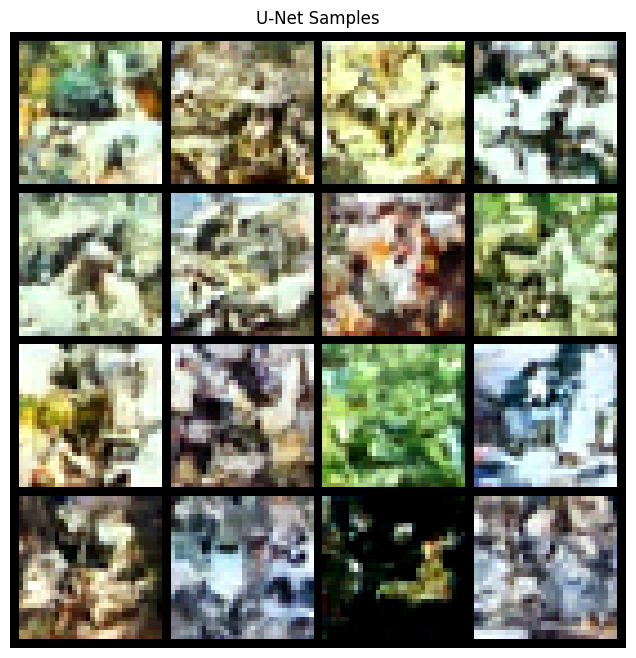
\includegraphics[width=0.48\linewidth]{figs/unet_samples.png}
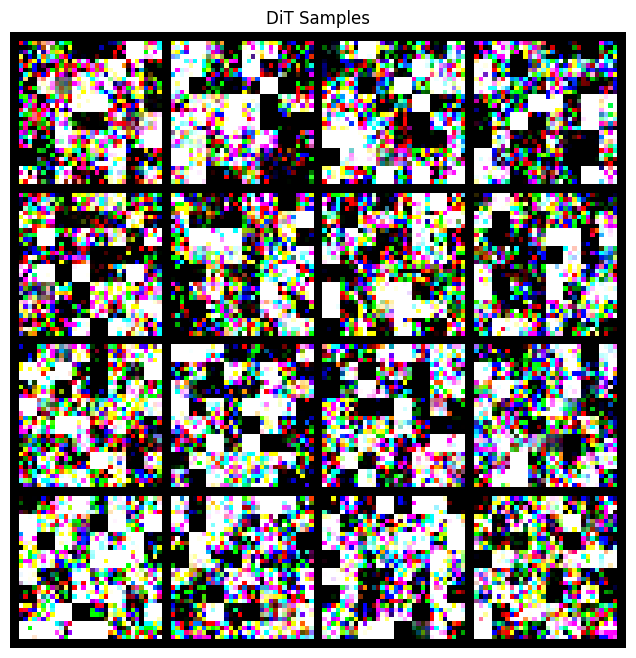
\includegraphics[width=0.48\linewidth]{figs/dit_samples.png}
\label{fig:samples}

Representative samples generated by the EMA models after $40$ epochs of training.
The U-Net produces recognizable CIFAR-10-like images with coherent structure, while the DiT samples exhibit more noise and less spatial coherence, consistent with its higher training loss.


\section{Ablation Studies}

\paragraph{Patch size.}
\Cref{tab:ablation-patch} shows DiT performance across patch sizes $2$, $4$, and $8$.
The default $p=4$ ($64$ tokens) performs best across all metrics.
Reducing to $p=2$ ($256$ tokens) worsens performance (despite finer resolution), likely because the quadratic attention cost over $256$ tokens makes training harder within the same budget.
Increasing to $p=8$ ($16$ tokens) collapses performance: the final loss of $0.353$ is close to untrained, indicating that $16$ tokens provide insufficient spatial resolution for denoising $32\times 32$ images.
\begin{table}[H]
    \caption{Patch-size ablation for the DiT. All variants trained for 50 epochs with depth $4$ and hidden dimension $128$. Patch size $4$ provides the best trade-off between token count and spatial resolution.}
    \label{tab:ablation-patch}
    \centering
    \begin{tabular}{cccccc}
    \toprule
    Patch Size & Tokens & Final Loss & Masked MSE & Unmasked MSE \\
    \midrule
    2 & 256 & 0.160 & 1.776 & 1.110 \\
    4 & 64 & \textbf{0.079} & \textbf{1.182} & \textbf{0.566} \\
    8 & 16 & 0.353 & 3.657 & 2.901 \\
    \bottomrule
    \end{tabular}
\end{table}

\paragraph{Depth.}

\Cref{tab:ablation-depth} shows the effect of increasing the DiT depth from $4$ to $6$ and $8$ transformer blocks.
Increasing depth improves performance relative to depth-$4$ baseline: the final loss decreases from $0.0791$ to $0.0779$, and the masked-region MSE decreases from $1.205$ to $1.167$.
However, the improvement saturates quickly.
Moving from depth $6$ to depth $8$ produces almost no additional gain.

This suggests that, in our small-scale setting, additional transformer depth helps up to a point but does not close the gap with the U-Net.
The bottleneck is therefore unlikely to be depth alone.
Instead, the DiT may need either substantially more scale, longer training, or architectural changes such as multi-resolution processing and skip connections to become competitive with the convolutional baseline.

\begin{table}[H]
    \caption{Depth ablation for the DiT. All variants use patch size $4$ and hidden dimension $128$. Increasing depth from $4$ to $6$ improves performance slightly, but gains saturate by depth $8$.}
    \label{tab:ablation-depth}
    \centering
    \begin{tabular}{cccc}
    \toprule
    Depth & Final Loss & Masked MSE & Unmasked MSE \\
    \midrule
    4 & 0.0791 & 1.205 & 0.570 \\
    6 & 0.0779 & \textbf{1.167} & \textbf{0.545} \\
    8 & \textbf{0.0778} & 1.168 & 0.548 \\
    \bottomrule
    \end{tabular}
\end{table}


\section{Implementation Details}
\label{app:implementation}
All code is implemented in PyTorch.
Both models are trained on a single GPU using mixed-precision training.


\end{document}
